\documentclass[../main.tex]{subfiles}
\graphicspath{
    {"../img/"}
    {"img/"}
}

\begin{document}
    \[
        \int\limits_{\partial D}f(z) dz = 2\pi i \sum_{z_k}^{} \Res_{z=z_k}f(z)
    .\]
\begin{przyklad}
    \[
        J = \int\limits_0^{2\pi} \frac{dx}{1-2a\cos(x) + a^2},\quad 0 < a < 1
    .\]
Niech $z = e^{ix}$, $dz = ie^{ix}dx$.
\[
    1-2a\cos(x) + a^2 = \frac{1}{z}\left(z-az^2-a+a^2z\right) = \frac{1}{z}(1-az)(z-a)
.\]
\[
    J = \int\limits_0^{2\pi} \frac{z dx}{(1-az)(z-a)} = \int\limits_{\partial K(0,1)} \frac{z}{(1-az)(z-a)} \frac{1}{i}\frac{dz}{z} = \frac{1}{i}\int\limits_{\partial K(0,1)} \frac{dz}{(1-az)(z-a)}
,\]
ale
\[
    \int\limits_{\partial K(0,1)} \frac{dz}{(1-az)(z-a)} = 2\pi i \underset{z=a}{\Res} f(z)
.\]
Zauważmy, że $(z-a)f(z)$ jest regularne w $z=a$, bo wynosi $\frac{1}{1-az}$.\\
Zatem
\[
    \underset{z=a}{\Res} f(z) = \lim\limits_{z\to a} \frac{z-a}{(z-a)(1-az)} = \lim\limits_{z\to a} \frac{1}{(1-az)} = \frac{1}{1-a^2}
.\]
Wychodzi
\[
    J = \frac{1}{i}2\pi i \frac{1}{1-a^2} = \frac{2\pi}{1-a^2}
.\]
\end{przyklad}
\textit{Czyli jest ładnie i słodko}\\
Wiemy, że jeżeli $f$ ma biegun stopnia $n$ w $z = z_k$, to
\[
    \lim\limits_{z\to z_k} (z-z_k)^{n} f(z)
\]
będzie wiekością skończoną, bo $f(z) = \sum_{n=0}^{\infty} a_n (z-z_k)^n + \frac{a_{-1}}{(z-z_k)} + \ldots + \frac{a_{-n}}{(z-z_k)^n}$

\begin{pytanie}
    Jak zachowuje się funkcja gdy $z_0$ jest punktem istotnie osobliwym?
\end{pytanie}
\begin{przyklad}
    Weźmy
    \[
        f(z) = e^{\frac{1}{z}}
    .\]
Wtedy
\[
    f(z) = \sum_{n=0}^{\infty} \left( \frac{1}{z} \right) ^n \frac{1}{n!}
.\]
Zbadamy
\[
    \lim\limits_{z\to 0}f(z)
.\]
\[
    \lim\limits_{r\to 0}f\left( re^{i\varphi} \right) = \lim\limits_{r\to 0}e^{\frac{1}{re^{i\varphi}}} = \lim\limits_{r\to 0} e^{\frac{1}{r}\cdot e^{-i\varphi}} = \lim\limits_{r\to 0}e^{\frac{1}{r}(\cos \varphi - i\sin\varphi)} = \lim\limits_{r\to 0}e^{-i \cdot \frac{1}{r} \sin\varphi}\cdot e^{\frac{1}{r}\cos\varphi}
.\]
A to dla $\cos\varphi > 0$ idzie do $+\infty$, dla $\cos\varphi < 0$ idzie do $0$, a dla $\cos\varphi = 0$ nie wiadomo. Stąd wiadomo, że granica nie istnieje.
\end{przyklad}
\begin{przyklad}
    \[
        J = \int\limits_{-\infty}^{+\infty} R(x)dx
    ,\]
gdzie $R : \mathbb{R}\to \mathbb{R}$ takie, że
\begin{enumerate}
    \item $R(z)$ nie ma biegunów na osi rzeczywistej
    \item $z\cdot  R(z) \underset{|z| \to +\infty}{\longrightarrow} 0$
\end{enumerate}
np.
\[
    J = \int\limits_{-\infty}^{+\infty} \frac{dx}{(x^2 + 1)^3}
.\]
Obszar - półokrąg o promieniu $r$.
Policzmy
\[
    \int\limits_{-r}^{r}R(x)dx
.\]
Weźmy funkcję $R(z)$ i policzmy
\[
    \int\limits_{\partial D}R(z)dz = \int\limits_{-r}^{r}R(x)dx + \int\limits_{C_r}R(z)dz = 2\pi i \sum \underset{z_k \in D}{\Res} f(z)
.\]
Jeżeli pokażemy, że
\[
    \lim\limits_{r\to\infty}\int\limits_{C_r}R(z)dz \to 0
\]
to będzie z głowy.
\[
    \int\limits_{C_r}R(z)dz = \int\limits_{0}^{\pi} re^{i\varphi}R(re^{i\varphi}) d\varphi = J_1
,\]
ale
\[
    \left| J_1 \right| \le \underset{0\le\varphi\le\pi}{\max}\left| r R(re^{i\varphi}) \right| \pi \to 0
,\]
bo założyliśmy, że $z R(z) \underset{|z| \to +\infty}{\longrightarrow} 0$.
\end{przyklad}
\begin{przyklad}
    Transformata Legendre'a geometrycznie\\
    niech np. $f(x) = x^2$.\\
    Wiemy, że
    \[
        p = \frac{\partial f}{\partial x} = 2x,\quad x = \frac{p}{2}
    \]
    \begin{align*}
        p &= \frac{f(x) - \psi(p)}{x}\\
        px &= f(x) - px\\
        \psi(p) &= \left(\frac{p}{2}\right)^2 - p \left(\frac{p}{2}\right)\\
        y &= px - \frac{p^2}{4}
    .\end{align*}
    I ogólnie
    \[
        f(x) \to p = \frac{\partial f}{\partial x} (x) \to x(p) = \left( \frac{\partial f}{\partial x}  \right) ^{-1}(p)
    .\]
Więc
\[
    \psi(p) = f(x(p)) - px(p)
.\]
\end{przyklad}
\begin{figure}[h]
    \centering
    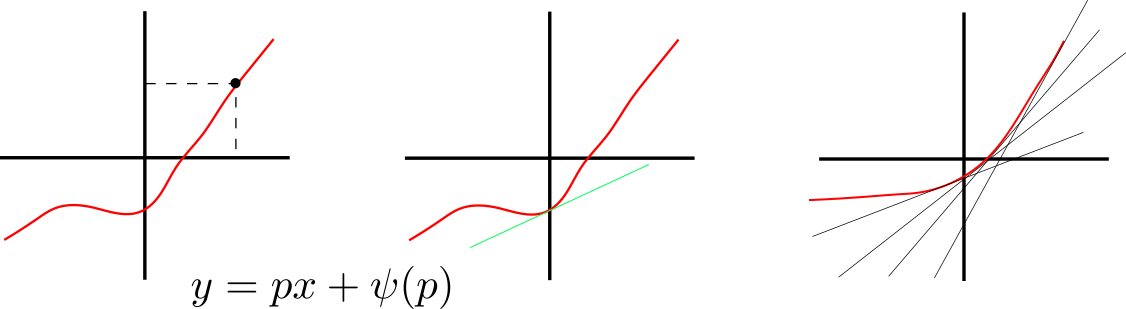
\includegraphics[width=0.8\textwidth]{w14-1.png}
\end{figure}

\begin{przyklad}
    Funkcja $L(q,\dot{q})$.
     \[
         p = \frac{\partial L}{\partial \dot{q}} \implies (\dot{q}) = \left( \frac{\partial L}{\partial \dot{q}}  \right) ^{-1} (p)
    .\]
Teraz szukamy $\psi(p)$, ale $\psi$ to jest $H$.
\[
    H(q,p) = L(q,\dot{q}) - p\cdot \dot{q}
.\]
\end{przyklad}
\begin{przyklad}
    \[
        \frac{d}{dt}\left( \frac{\partial L}{\partial \dot{q}}  \right) - \frac{\partial L}{\partial q} = 0 \implies \frac{\partial L}{\partial q} = \dot{p}
    .\]
\end{przyklad}
Jeżeli $\psi(p) = f(x(p)) - px(p)$, to
\[
    d\psi(p) = \left(\frac{\partial f}{\partial x} \cdot \frac{\partial x}{\partial t} - x(p) - p \frac{\partial x}{\partial p} \right)dp
,\]
ale $\frac{\partial f}{\partial x} = p$, czyli
\[
    d \psi(p) = -x(p) dp
.\]
Ale zazwyczaj jest tak
\[
    d\psi(p) = \frac{\partial \psi}{\partial p} dp
.\]
czyli powinno być
\[
    -x(p) = \frac{\partial \psi}{\partial p}
.\]
Wracając do przykładu 4, mamy $\psi(p) = -\frac{p^2}{4} \implies -x(p) = -\frac{p}{2} \implies p = 2x$.
Ale
\[
    \psi(p) = f(x) - px \implies f(x) = \frac{-(2x)^2}{4}+ 2x x = -x^2 + 2x^2 = x^2
.\]
\begin{przyklad}
    Mamy gaz i funkcję stanu $U(V,N,S)$. Możemy zrobić z niej jednoformę
     \[
    dU = \frac{\partial U}{\partial V} dV + \frac{\partial U}{\partial N} dN + \frac{\partial U}{\partial S} dS
    .\]
Albo nawet dd
\[
    ddU = \left( \frac{\partial }{\partial S} \left( \frac{\partial U}{\partial V}  \right) - \frac{\partial }{\partial V} \left( \frac{\partial U}{\partial S}  \right)  \right) ds\land dv = 0
.\]
Można jeszcze dalej, zupgradować którąś pochodną na zmienną niezależną. Niech $\frac{\partial U}{\partial S} = T$. Dostajemy nową funkcję (energia swobodna Helmholtza) $F(V,N,T) = U - T\cdot S$.
\[
    \frac{\partial U}{\partial V} = -p,\quad H(p,N,S) = U + pV
.\]
I później wychodzi
\[
    - \frac{\partial P}{\partial S} - \frac{\partial T}{\partial V} = 0
.\]
\end{przyklad}

\end{document}
